%% CS 567 - 3D User Interfaces and Human-Centered Spatial AI - Fall 2026
%% Project Proposal template.
%%
%% This is the LaTeX twin of CS567-Proposal-Template.docx. Same sections, same
%% guidance, same checklist -- use whichever you prefer. Compiles on Overleaf
%% (Professional is free for CSU students) with pdfLaTeX.
%%
%% Deliberate departures from stock acmart sigconf:
%%   * nonacm: this is a class proposal, not an ACM submission, so the
%%     copyright block, the conference line and the CCS concepts are all off.
%%   * The seven required proposal items are real sections, so the document you
%%     fill in already has the shape of your final paper.
%%   * Guidance text is gray italic and marked for deletion (\guide{...}).

\documentclass[sigconf,nonacm]{acmart}

\settopmatter{printacmref=false, printccs=false, printfolios=true}
\setcopyright{none}
\acmConference{CS 567: 3D User Interfaces and Human-Centered Spatial AI}{Fall 2026}{Colorado State University}

\usepackage{xcolor}
\usepackage{graphicx}
\usepackage{booktabs}
\usepackage{tabularx}

%% Gray italic instruction text. DELETE every \guide{...} before you submit.
\newcommand{\guide}[1]{{\color{gray}\itshape #1\par\medskip}}

\begin{document}

%% ---------------------------------------------------------------- title
\title{Local-First: Human-Centered  Routing Between Local and Frontier Language Models}
\subtitle{CS567-Local-First-AI}
\author{Kaleb Flowers}
\email{Kaleb.Flowers@colostate.edu}
\affiliation{%
  \institution{Colorado State University}
  \department{Department of Computer Science}
  \city{Fort Collins}
  \state{CO}
  \country{USA}}

\renewcommand{\shortauthors}{CS567-Local-First-AI}

%% ---------------------------------------------------------------- abstract
\begin{abstract}
As the use of large cloud based language models continues to grow, concerns about energy consumption, privacy, network dependence, and unnecessary use of computational resources make local inference increasingly important. Local-First investigates whether programming tasks can be routed between local and frontier language models in a way that reduces dependence on cloud based models without meaningfully reducing task performance. The system will support both human model selection and agentic model selection through a shared programming task interface. A locally running routing agent will decide whether each task should remain on device or be escalated to a frontier model. The evaluation will compare task success, frontier-model usage, local task success, routing failures, response latency, and participant workload. Human and agentic selection will also be compared against always-local and always-frontier baselines. The goal is to determine whether agentic routing can preserve successful task completion while shifting more work to local models.
\end{abstract}

\keywords{human-centered AI; agentic AI; model routing; local inference; on-device inference; small language models; frontier models}

\maketitle


%% ---------------------------------------------------------------- body
\section{Introduction and Motivation}
Large language models are increasingly available through both powerful cloud services and smaller models that can run directly on consumer hardware. Frontier models provide strong performance across a wide range of tasks, but relying on them for every interaction comes with costs in energy use, privacy, network dependence, latency, and monetary expense. Data centers already account for more than 2\% of annual U.S. energy consumption, and the growing use of language models adds to that demand. At the same time, smaller language models require fewer resources and can run locally on everyday devices, while still performing well on more straightforward tasks. The problem is that users generally have no clear way to know when a local model is capable enough for a task and when a frontier model is actually necessary. This is not a simple distinction because the capability of the local model varies with the model, hardware, and task. The difficulty of a request is not always obvious from the prompt itself. As a result, users may default to much larger cloud models even for tasks that could be completed satisfactorily on their own device. Determining when local inference is sufficient could reduce unnecessary reliance on frontier models without sacrificing the quality of the user experience.  

\section{Related Work}
\noindent\textbf{Adaptive LLM Routing}\par
\noindent Recent work has shown that not every request needs to be handled by the largest or most capable language model. Existing approaches differ in when the routing decision is made and what information is used to make it. FrugalGPT uses a cascading approach where models are called sequentially and the quality of each response is evaluated before deciding whether another model is needed~\cite{chen2024frugalgpt}. Hybrid LLM makes the routing decision before inference by predicting whether a smaller model can provide sufficient response quality or whether the request should be sent to a stronger, more capable model. This approach reduced calls to the larger model by as much as 40\% without reducing response quality~\cite{ding2024hybridllm}. Ong et al. also routes between weaker and stronger models before inference, but their routers are trained using human preference data rather than only generated quality labels~\cite{ong2025routellm}. BEST-Route extends the routing decision further by selecting both which model should handle a request and how much test time computation should be allocated to it, this allows additional computation on smaller models to avoid using the strongest model~\cite{ding2025bestroute}. Pozi and Sato apply pre-inference routing specifically to program generation, using a lightweight classifier to route prompts between a weaker edge model and a stronger cloud model~\cite{pozi2025routing}. Together this work demonstrates several ways to reduce unnecessary use of stronger models while preserving response quality. Even when human preference data is used to train the router, the model-selection decision is still made automatically at runtime. 

\noindent\textbf{Local and Cloud Inference}\par
\noindent Model routing becomes particularly important when the available models run in different environments. Hybrid LLM describes a setting in which smaller models can execute on laptops or mobile devices while more difficult requests are sent to a cloud API~\cite{ding2024hybridllm}. Pozi and Sato evaluate this type of edge-cloud architecture for program generation, routing simpler prompts to a weaker edge model and more difficult prompts to a stronger cloud model~\cite{pozi2025routing}. Research on smaller models also supports the feasibility of local execution. MobileLLM demonstrates that sub-billion-parameter models designed for on-device use can remain useful for common language tasks and achieve performance approaching much larger models on API-calling tasks~\cite{liu2024mobilellm}. Jeanquartier et al. examine the resource and environmental effects of language-model deployment and identify smaller models as a practical option for straightforward and resource-constrained workloads, including execution on everyday devices~\cite{jeanquartier2026carbon}. Agent-X approaches local execution from an agentic systems perspective and demonstrates an AI agent operating entirely on-device while also identifying latency as an important limitation of resource-constrained hardware~\cite{chung2026agentx}. These studies show that local inference can be a practical execution option, but its usefulness depends on matching the capability of the local model and hardware to the requirements of the task.

\noindent\textbf{Context-Aware and Agentic LLM Systems}\par
\noindent LLM-based systems can also incorporate information beyond the user's immediate request when reasoning about how a task should be handled. Hallgarten et al. demonstrate this with RouteLLM, which incorporates route context such as road conditions, traffic, and weather into the model's reasoning process~\cite{hallgarten2025routllm}. Their work also evaluates the system through a comparative user study, illustrating how context-aware LLM systems can be studied from both system and user perspectives. Agentic systems extend this idea by allowing an LLM to make decisions about how a task should be completed. HuggingGPT demonstrates this approach by using an LLM to plan a task and select other models to carry out the required work~\cite{shen2023hugginggpt}. This shows that model selection can itself become part of an agent's decision-making process rather than being fixed in advance. 

Across the work reviewed here, model routing, local inference, context-aware reasoning, and agentic resource selection have each been demonstrated, but none of these studies directly compares a user's local-versus-frontier model choice with an agent's choice while holding the task and execution pipeline constant. Local-First addresses this gap by comparing two selection conditions for the same programming tasks: one in which the participant chooses whether a request should be handled locally or by a frontier model, and one in which a locally running routing agent makes that decision. This design shifts the question from whether model routing is technically possible to whether an agentic routing process can make effective local-first decisions relative to users themselves, while maintaining task success, avoiding unnecessary reliance on frontier models, and examining how the selection method affects user satisfaction.

\section{Approach}
This project will use two complementary approaches to study model orchestration. 
\begin{itemize}
\item \textbf{Human model selection:} Participants will be given programming tasks and access to both a local model and a frontier model. They will choose which model to use for each task, allowing me to study how people make model selection decisions when both options are available.
\item \textbf{Agentic model selection:} An automated agent will examine each task and decide whether it should be handled locally or escalated to a frontier model. The decisions made by the agent will then be compared with those made by the participants.\end{itemize}

\section{System Vision and Technology}
\noindent
Local-First will provide a programming task workspace with a task panel, model selection controls, and a response area. In human-selection mode, the participant will choose Local or Frontier before submitting the task. In agentic selection mode, a locally running routing agent will make that choice. Both modes will use the same layout and response controls. The interface will show the selected model, request progress, and returned explanation and code, with attention to readability and clear interaction states. Figure~\ref{fig:mockup} shows the proposed interface for both selection modes.

The routing agent will determine whether the available local model is likely sufficient for a task or whether a frontier model is needed. It may consider the task, information about the local model’s capabilities, and hardware specification. The exact decision method remains open. Routing will happen locally before task execution. Both selection modes will use a shared execution layer and a common model interface to access either Ollama or a frontier-model API (potentially OpenAI or Anthropic). Responses will be returned in a consistent format without rewriting their content for evaluation. Logging throughout the process will record tasks, selections, responses, timestamps, and errors. Figure~\ref{fig:architecture} shows the proposed system architecture and the shared execution path used after model selection.

The proposed implementation will tentatively use Python for orchestration and NiceGUI for the browser based interface, with FastAPI underlying the application. Ollama will provide local inference, while a cloud API will provide access to the frontier-model. The exact models and demonstration machine will be selected during prototyping.


\section{Evaluation Plan}
\noindent
The evaluation will test whether agentic local-first routing can reduce
reliance on frontier models while maintaining comparable programming task
performance to human model selection. The primary independent variable will
be selection mode: human selection or agentic selection. The primary
hypothesis is that agentic routing will reduce frontier-model usage without
causing a meaningful decrease in task success. A secondary hypothesis is that
agentic selection will reduce participant workload.

\begin{table}[htbp]
\centering
\caption{Evaluation measures}
\label{tab:evaluation}
\small
\begin{tabularx}{\columnwidth}{@{}p{0.38\columnwidth}X@{}}
\toprule
\textbf{Measure} & \textbf{Purpose} \\
\midrule
Task success &
Successful task completion. \\

Frontier usage &
Reliance on frontier inference. \\

Local task success &
Tasks completed entirely locally. \\

Avoidable frontier use &
Unnecessary escalation to the frontier model. \\

Failed local routing &
Local selections that fail when frontier inference succeeds. \\

Response latency &
End-to-end response time. \\

NASA-TLX &
Participant-reported workload. \\

Preference &
Preferred selection mode. \\
\bottomrule
\end{tabularx}
\end{table}

\noindent
\begin{minipage}{\columnwidth}
Task success and frontier usage will serve as the primary system-level
outcomes and will be considered together. A successful routing strategy should
reduce frontier-model usage without meaningfully reducing task success.
Always-local and always-frontier execution will also be evaluated as system
baselines. Programming tasks will span a range of difficulty levels, with
correctness measured using task specific tests when possible and a scoring
rubric when automated testing is insufficient.\end{minipage}

Participants will be users with programming experience, with recruitment likely focused on computer science students. Participants should have enough experience to understand the programming tasks and make meaningful model selection decisions, but they will not need expert level programming knowledge. The study will be conducted as an internal class project, with the required human participant submission completed before data collection.

\section{Deliverables}
\label{sec:deliverables}
By mid-November, the project will include:

\begin{itemize}
    \item A working Local-First prototype with a browser based programming task interface, human-selection mode, agentic-selection mode, local inference through Ollama, frontier-model access through a cloud API, and logging of routing decisions, responses, latency, and errors.
    
    \item A local routing agent that decides whether each programming task should remain on-device or be escalated to a frontier model.
    
    \item A study dataset containing task-success results, local and frontier-model usage, avoidable frontier use, failed local routing, response latency, participant workload measured with NASA-TLX, and overall selection-mode preference.
    
    \item An analysis comparing human selection, agentic selection, always-local execution, and always-frontier execution, with emphasis on whether agentic routing reduces frontier-model usage while maintaining comparable task success.
    
    \item A final research paper describing the system, related work, study design, results, limitations, and conclusions.
    
    \item Status, prototype, and final demonstration videos showing the implementation, study progress, and final system behavior.
\end{itemize}

As the sole member of CS567-Local-First-AI, I will be responsible for the system design, implementation, participant study, data collection and analysis, paper, and presentation materials.

\section{Conclusion}
Local-First will examine whether agentic routing can reduce reliance on frontier language models while maintaining comparable performance on programming tasks. The project will compare human and agentic model selection using the same interface and evaluate both system performance and participant workload. The final system will include a working local-first prototype, study data, and an analysis of how much work can remain local before frontier inference becomes necessary.

\section*{Use of AI}
Generative AI was used to help identify relevant literature, evaluate the organization and clarity of the arguments, and review and revise grammar and phrasing for clarity. The final text, citations, and technical claims were reviewed by the author.  

\begin{figure*}[p]
  \centering
  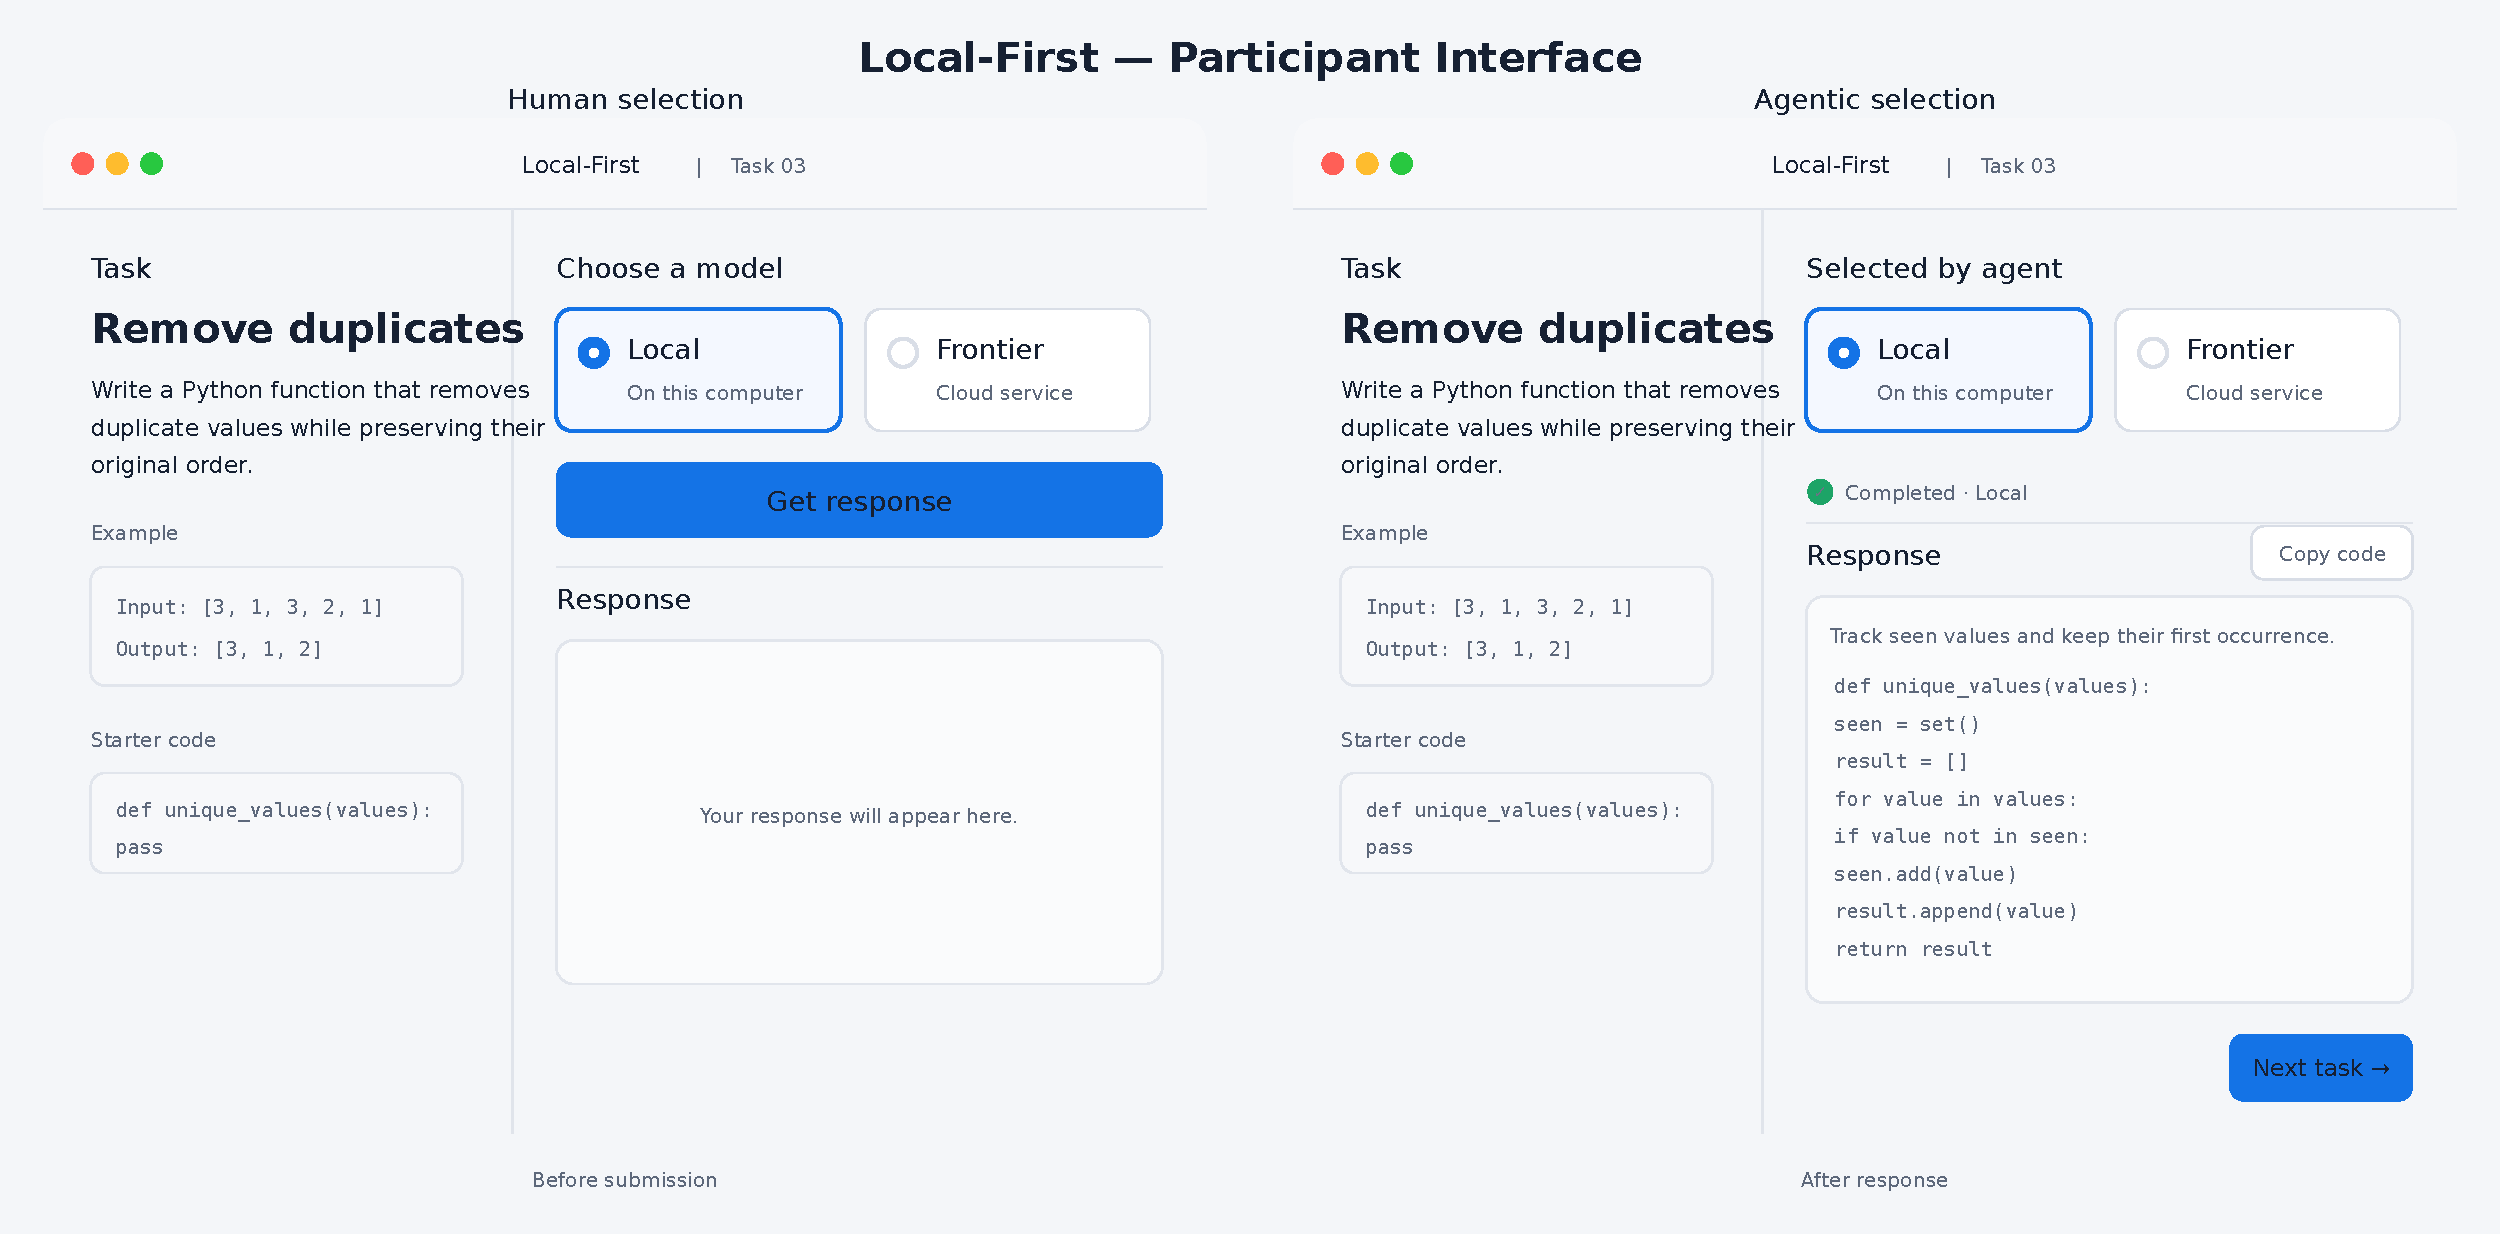
\includegraphics[width=\textwidth]{local-first-interface-mockup.pdf}
  \caption{Proposed Local-First participant interface. In human-selection
  mode, the participant chooses between local and frontier inference. In
  agentic-selection mode, the interface displays the route chosen by the
  local routing agent. Both modes use the same task and response layout.}
  \label{fig:mockup}
\end{figure*}

\begin{figure*}[p]
  \centering
  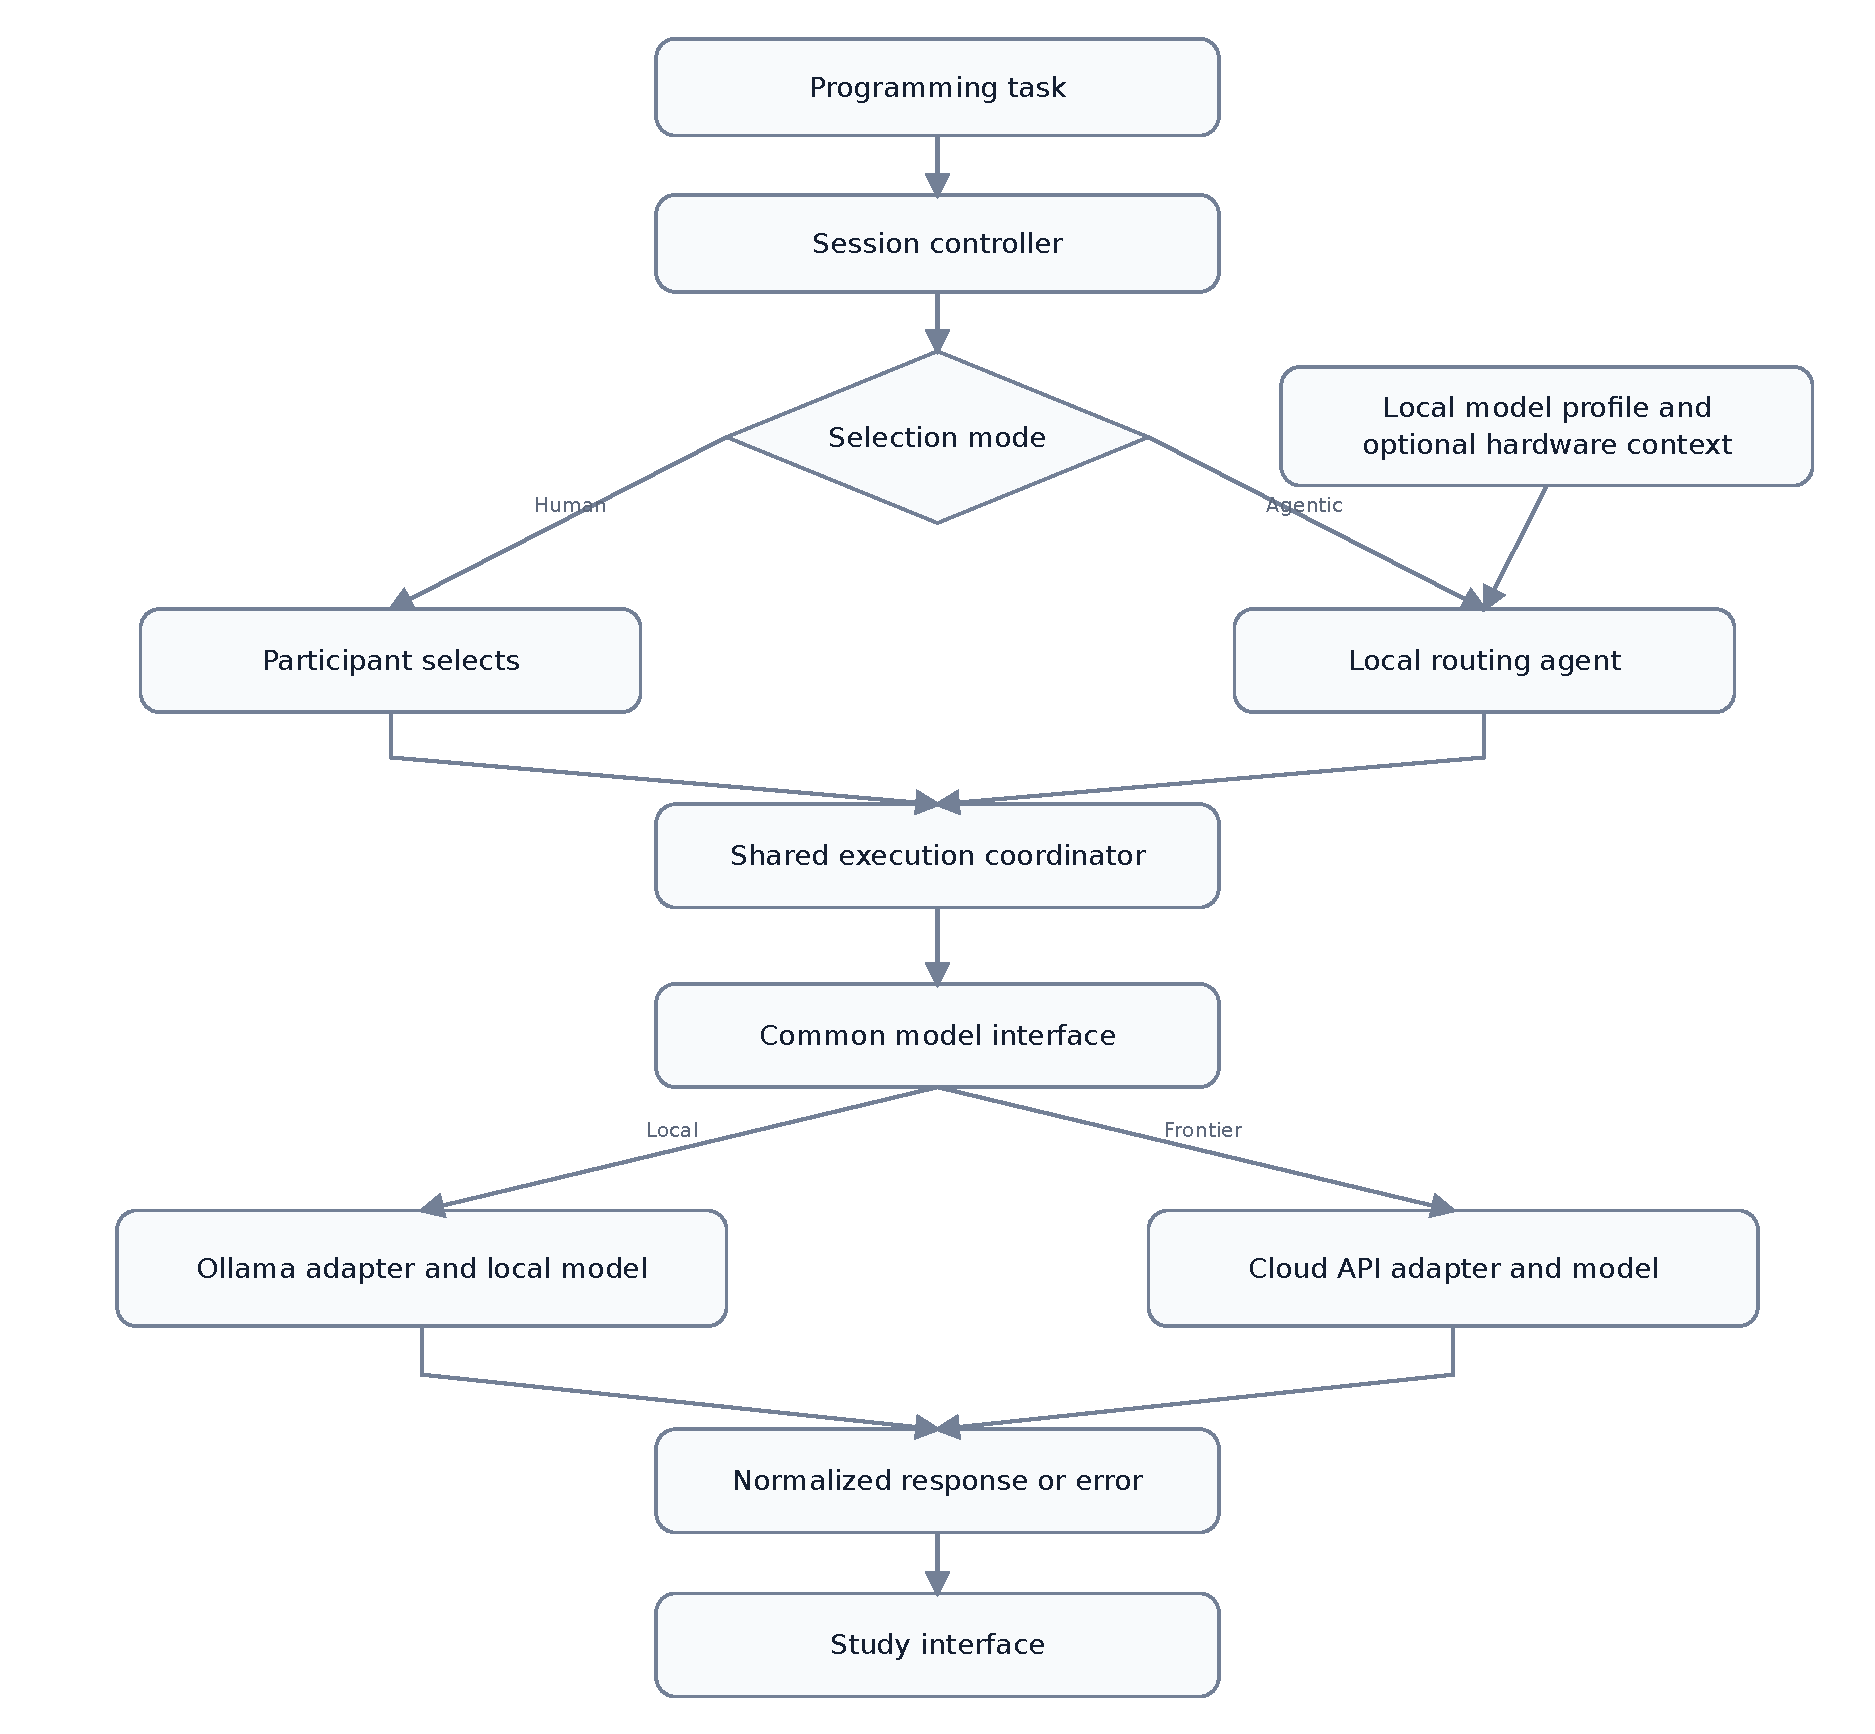
\includegraphics[width=0.88\textwidth]
  {local-first-system-flowchart.pdf}
  \caption{Proposed Local-First system architecture. Human and agentic
  selection use different decision paths but share the same execution and
  model-access components after a route is selected.}
  \label{fig:architecture}
\end{figure*}

\clearpage

%% ---------------------------------------------------------------- references

\bibliographystyle{ACM-Reference-Format}
\bibliography{references}

\end{document}
